\documentclass[11pt]{jarticle}
\usepackage{ITCannual}
\usepackage{amsmath}
\usepackage{amssymb}
\usepackage{times}
\usepackage{graphicx}

%\usepackage[style=numeric]{biblatex}



\title{データ科学研究部門 研究報告}
\author{小林博樹, 松島慎, 中村覚, 姜仁河, 川瀬純也, 石川正俊, 早川智彦, 黄守仁, 末石智大, 宮下令央, 他8名}

\begin{document}
\maketitle

\section{データ科学研究部門 概要}
...



\subsection{2020年度石川研究室全体の研究活動概要}
現実の物理世界は, 原則的に並列かつリアルタイムの演算構造を有している. その構造と同等の構造を工学的に実現することは, 現実世界の理解を促すばかりでなく, 応用上の様々な利点をもたらし, 従来のシステムをはるかに凌駕する性能を生み出すことができ, 結果として, まったく新しい情報システムを構築することが可能となる.本研究室では,特にセンサ情報処理における並列処理と高速・リアルタイム性を高度に示現する研究として, 以下を行っている. また, 新規産業分野開拓にも力を注ぎ,研究成果の技術移転, 共同研究, 事業化等を様々な形で積極的に推進している.センサフュージョンの研究として、高速ビジョン等のセンサ情報に基づく高速知能ロボットの開発並びにその応用としての新規タスクの実現や人間機械協調システムの開発を行っている.ダイナミックビジョンシステムの研究では、高速ビジョンや能動光学系を用いて運動対象の情報を適応的に取得する基礎技術及びトラッキング撮像等の応用システムの開発を行っている.システムビジョンデザインの研究では、高速三次元計測や質感計測等の並列処理に基づく高速画像処理技術(理論、アルゴリズム、デバイス)の開発を行っている.アクティブパーセプションの研究として、高速ビジョンを用いた能動計測や能動認識の研究を行い、実世界における新たな知覚補助技術並びにそれに基づく新しい対話の形の創出を目指している.


\section{データ科学研究部門 成果要覧}
\begin{招待講演}{1}


\end{招待講演}

\begin{招待論文}{1}


\end{招待論文}

\begin{受賞}{1}

\bibitem{SatoruNakamura201} 
小風尚樹, 中村覚, 永崎研宣:
 情報処理学会 人文科学とコンピュータシンポジウム「じんもんこん2019」 学生奨励賞 構造化記述された財務記録史料データの分析手法の開発:イギリスの船舶解体業を事例に
\end{受賞}

\begin{著書}{1}

\bibitem{SatoruNakamura301} 
中村覚(担当:共編者(共編著者)):
 デジタルアーカイブ・ベーシックス 2:災害記録を未来に活かす, 2019年8月 (ISBN: 9784585202820)
\end{著書}

\begin{雑誌論文}{1}

\bibitem{JIANG1901}
Zipei Fan, Xuan Song, Renhe Jiang, Quanjun Chen, and Ryosuke Shibasaki:
Decentralized Attention-based Personalized Human Mobility Prediction, Proceedings of the ACM on Interactive Mobile Wearable and Ubiquitous Technologies, Vol.3, No.4, pp1-26, December 2019.
\bibitem{JIANG2001}
Zipei Fan, Xuan Song, Quanjun Chen, Renhe Jiang, Ryosuke Shibasaki, and Kota Tsubouchi:  
Trajectory fingerprint: one-shot human trajectory identification using Siamese network, CCF Transactions on Pervasive Computing and Interaction, 2(2), 113-125, 2020.
\bibitem{JIANG2002}
Renhe Jiang, Quanjun Chen, Zekun Cai, Zipei Fan, Xuan Song, Kota Tsubouchi, and Ryosuke Shibasaki: 
Will You Go Where You Search? A Deep Learning Framework for Estimating User Search-and-Go Behavior, Neurocomputing, 2020.
\bibitem{JIANG2003}
Renhe Jiang, Xuan Song, Zipei Fan, Tianqi Xia, Zhaonan Wang, Quanjun Chen, Zekun Cai, and Ryosuke Shibasaki: 
Transfer Urban Human Mobility via POI Embedding over Multiple Cities, ACM/IMS Trans. Data Sci. 2, 1, Article 4, 26 pages, January 2021.
\bibitem{LMY01}
T. Lee, S. Matsushima, K. Yamanishi: “Grafting for combinatorial binary model using frequent itemset mining,” Data Mining and Knowledge Discovery, 34(1), pp. 101-123 (2020)
\bibitem{FMY01}
Y. Fu, S. Matsushima, K. Yamanishi: “Model Selection for Non-Negative Tensor Factorization with Minimum Description Length,” Entropy 2019, 21, 632.
	
\end{雑誌論文}

\begin{査読付}{1}

\bibitem{JIANG1902}
Renhe Jiang, Xuan Song, Dou Huang, Xiaoya Song, Tianqi Xia, Zekun Cai, Zhaonan Wang, Kyoung-Sook Kim, and Ryosuke Shibasaki:
Deepurbanevent: A system for predicting citywide crowd dynamics at big events, Proceedings of The 25th ACM SIGKDD International Conference on Knowledge Discovery \& Data Mining (KDD'19), pp2114-2122, July 2019.
\bibitem{JIANG1903}
Zipei Fan, Quanjun Chen, Renhe Jiang, Ryosuke Shibasaki, Xuan Song, and Kota Tsubouchi:
Deep Multiple Instance Learning for Human Trajectory Identification, Proceedings of the 27th ACM SIGSPATIAL International Conference on Advances in Geographic Information Systems (SIGSPATIAL'19), pp512-515, November 2019.
\bibitem{JIANG1904}
Xiaodan Shi, Xiaowei Shao, Zipei Fan, Renhe Jiang, Haoran Zhang, Zhiling Guo, Guangming Wu, Wei Yuan, and Ryosuke Shibasaki:
Multimodal Interaction-Aware Trajectory Prediction in Crowded Space, Proceedings of The Thirty-Fourth AAAI Conference on Artificial Intelligence (AAAI'20), pp11982-11989, February 2020.
\bibitem{JIANG2004}
Satoshi Miyazawa, Xuan Song, Renhe Jiang, Zipei Fan, Ryosuke Shibasaki, and Taisei Sato:
City-Scale Human Mobility Prediction Model by Integrating Gnss Trajectories and Sns Data Using Long Short-Term Memory, ISPRS Annals of the Photogrammetry, Remote Sensing and Spatial Information Sciences, Volume V-4-2020, 2020, pp.87-94, August 2020.
\bibitem{JIANG2005}
Quanjun Chen, Renhe Jiang, Chuang Yang, Zekun Cai, Zipei Fan, Kota Tsubouchi, Xuan Song, Ryosuke Shibasaki: 
DualSIN: Dual Sequential Interaction Network for Human Intentional Mobility Prediction, Proceedings of the 28th International Conference on Advances in Geographic Information Systems (SIGSPATIAL '20), pp.283–292, November 2020.
\bibitem{JIANG2006}
Xiaodan Shi, Xiaowei Shao, Guangming Wu, Haoran Zhang, Zhiling Guo, Renhe Jiang, Ryosuke Shibasaki: 
Social-DPF: Socially acceptable distribution prediction of futures, Proceedings of The Thirty-Fifth AAAI Conference on Artificial Intelligence (AAAI'21), February 2021.
\bibitem{HSM02}
S. Hayashi, M. Sugiyama, S. Matsushima: “Coordinate Descent Method for Log-linear Model on Posets,”  In Proceedings of IEEE International Conference on Data Science and Advanced Analytics (DSAA), pp. 99-108 (2020)
\bibitem{MB01}
S. Matsushima, M. Brbić: “Selective Sampling-based Scalable Sparse Subspace Clustering,” Advances in Neural Information Processing Systems (NeurIPS). pp. 12416-12425 (2019)
\bibitem{RSMZYV01}
P. Raman, S. Srinivasan, S. Matsushima, X. Zhang, H. Yun, S. V. N. Vishwanathan: “Scaling Multinomial Logistic Regression via Hybrid Parallelism,” ACM SIGKDD Conference on Knowledge Discovery and Data Mining (KDD), pp. 1460-1470 (2019)

\bibitem{SatoruNakamura401} 
中村覚, 佐治奈通子, 永崎研宣:
 TEI とIIIF をベースとしたオン/オフライン併合型史料研究支援システムの開発 - オスマン・トルコ語文書群を対象として,  じんもんこん2019論文集 2019 pp.293-300 2019.

\bibitem{SatoruNakamura402} 
小風尚樹, 中村覚, 永崎研宣:
 構造化記述された財務記録史料データの分析手法の開発:イギリスの船舶解体業を事例に,  じんもんこん2019論文集 2019 pp.183-190 2019.

\bibitem{SatoruNakamura403} 
Satoru Nakamura, Kazuhiro Okada, Kiyonori Nagasaki:
 An Attempt of Dissemination of TEI in a TEI-underdeveloped country: Activities of the SIG EAJ,  The 19th annual Conference and Members Meeting of the Text Encoding Initiative Consortium 2019.

\bibitem{SatoruNakamura404} 
Kazuhiro Okada, Satoru Nakamura, Kiyonori Nagasaki:
 An Encoding Strategic Proposal of “Ruby” Texts: Examples from Japanese Texts,  The 19th annual Conference and Members Meeting of the Text Encoding Initiative Consortium 2019.

\bibitem{SatoruNakamura405} 
Satoru Nakamura:
 Approach to develop Digital Collection for Small Organization considering Sustainability and Reusability with IIIF and Static File,  The 9th International Conference of Japanese Association for Digital Humanities pp.76-78 2019.

\end{査読付}

\begin{公開}{1}

\end{公開}

\begin{特許}{1}


\end{特許}

\begin{発表}{1}

\bibitem{KM01} 上月正貴、松島慎「二変数間の相互作用を考慮した一般化加法モデルの効率的な学習」第22回情報論的学習理論ワークショップ、名古屋、2019年11月
\bibitem{HSM01} 林翔太、杉山麿人、松島慎「半順序構造上の対数線形モデルのための座標降下法」第22回情報論的学習理論ワークショップ、名古屋、2019年11月
\bibitem{NM01} 西本洋紀、松島慎「対数線形モデルを基とした生成的分類器と識別的分類器のロジスティック汎化誤差の収束の比較」第23回情報論的学習理論ワークショップ、オンライン、2020年11月
\bibitem{KM02} 上月正貴、松島慎「二変数間相互作用を考慮した一般化加法モデルとその効率的な学習」科研費シンポジウム機械学習・統計学・最適化の数理とAI技術への展開、オンライン、2020年12月
\bibitem{SatoruNakamura701} 
中村覚, 水野遊大, 稗方和夫, 成田健太郎:
 デジタル文化資料活用システムの設計手法 ―法帖研究支援の事例― ,  人工知能学会研究会資料 SIG-KST-039-02 pp.1-6 2020.

\bibitem{SatoruNakamura702} 
NAKAMURA Satoru:
 Development of Content Retrieval System of Scrapbook “Kunshujo” using IIIF and Deep Learning,  2019 IIIF Conference 2019.

\bibitem{SatoruNakamura703} 
NAKAMURA Satoru, NAGASAKI Kiyonori:
 IIIF Discovery in Japan,  2019 IIIF Conference 2019.

\bibitem{SatoruNakamura704} 
佐治奈通子, 中村覚:
 歴史学と情報学のより良い協働を目指して―オープンなDH支援ツールを用いたボスニアのカトリック修道院所蔵のオスマン・トルコ語文書群のデータ整理の一事例,  研究報告人文科学とコンピュータ(CH) 2019-CH-120(11) pp.1-7 2019.

\bibitem{SatoruNakamura705} 
Ayano Kokaze, Satoru Nakamura, Kiyonori Nagasaki, Naoki Kokaze:
 Enriching the Life Cycle of data: Supporting a project by DH approach,  International Society for Eighteenth-Century Studies Congress 2019 2019.

\end{発表}

\begin{特記}{1}

\end{特記}

\begin{報道}{1}


\end{報道}


\section{データ科学研究部門 教員研究活動}

\subsection{研究報告(小林)}


\input{List/ITCannual-list-Kobayashi}

\subsection{研究報告(松島)}
本節では松島研究室の研究活動について報告する。
2019年度および2020年度に、弊研究室では解釈可能な機械学習手法の効率的な計算手法についての研究を推進してきた。

画像データや言語データを予測したり生成したり表層的に駆使することは可能になってきた。
しかしながら我々の画像や言語の理解が進んだわけではない。

機械学習は予測や分類など表層的なデータの駆使の方法論であるだけでなく、
データの関係を明らかにして人間の理解を助けるための方法論でもある。

特にデータ保持者の目線に立って機械学習を


成果は主に以下の3分野に大別される。
\begin{itemize}
    \item 一般化加法モデルに関する研究
    \item 組合せ線形モデルに関する研究
    \item 部分空間クラスタリングに関する研究
\end{itemize}

一般化加法モデルと組み合わせ線形モデルは
属性間の線形な関係を越えて、非線形な関係を抽出するための枠組みである。
部分空間クラスタリングはデータ集合が持つ単純な線形関係を超えて、
データのクラスタリングを行ってそれぞれのクラスタが持つ線形関係を抽出する枠組みである。


\subsubsection{一般化加法モデルに関する研究}
いわゆる線形モデルの学習とは以下のようにあらわされる
データの属性間の線形な関係を抽出する枠組みととらえることができる
\begin{align*}
    y = \sum_{j} w_j x_j
\end{align*}
データの属性$y$は通常予測したい変数であり、
他のデータ属性が$x_j$である。与えられたデータ集合を用いて$w_j$は実数全体から推定される。
一般化加法モデルでは以下のような関係を抽出する枠組みである
\begin{align*}
    y = \sum_{j} f_j (x_j)
\end{align*}
与えられたデータ集合を用いて$f_j$は(十分広い)関数クラス$F$から推定される。
このような$f_j$を推定できれば、例えば年齢と収入の非線形な関係などがデータから
学習できると考えられる。

最も単純な手法は$F$を推定の簡単さのために狭めの関数クラスに制限することである。
一般に与えられた基底関数集合$\left\{\varphi_k(\cdot):\mathbb{R} \to \mathbb{R} \right\}_{k=1,\ldots,K}$に対し
\begin{align*}
  F=\left\{  \sum_{k=1}^d \varphi_k(x_j) \right\}
\end{align*}
とすることはパラメトリックな手法と呼ばれる。
\cite{F}は〜\\

利用可能なデータ数に応じて関数クラスの大きさが変わる。
具体的にはデータ数が大きくなれば関数クラスも広くなっていくような手法をノンパラメトリックな手法と呼び、
そのような手法はカーネル法を使うよりなかった。
我々の手法はカーネル法よりも効率的に学習が可能である。


さらに複雑な関係性をデータから学習して可視化することが可能である
\begin{align*}
    y = \sum_{j,k} f_{j,k} (x_j,x_k)
\end{align*}




\subsubsection{組合せ線形モデルに関する研究}

組合せ線形モデルでは離散データ集合を考える。
離散データも多くの現実のデータを表現することができる。



\subsubsection{部分空間クラスタリングに関する研究}

部分空間クラスタリングにおい

\begin{figure}[h]
    \centering
    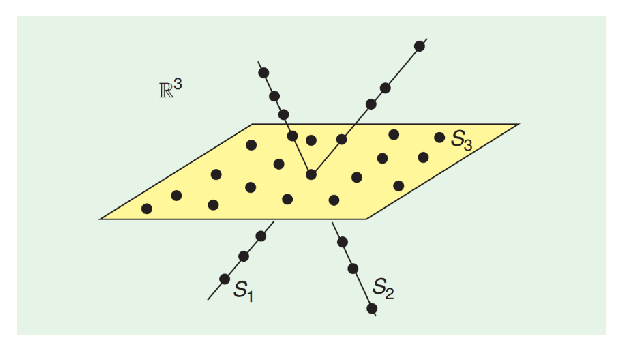
\includegraphics[width=7cm]{Matsushima/sc.eps}
    \caption{部分空間クラスタリングの3次元の例(\cite{SC}から抜粋)。距離が近い点同士ではなく、同じ平面上もしくは同じ直線上(部分空間上)にある点同士をクラスタとみなす。}
    \label{fig:my_label}
\end{figure}
\cite{HSM01}は〜\\
\cite{HSM02}は〜\\
\cite{KM01}は〜\\
\cite{KM02}は〜\\
\cite{NM01}は〜

\begin{thebibliography}{9}
\bibitem{F}
    Friedman, J., Hastie, T., & Tibshirani, R. (2010). 
    Applications of the lasso and grouped lasso to the estimation of sparse graphical models (pp. 1-22). Technical report, Stanford University.
\bibitem{SC}
 VIDAL, René. Subspace clustering. IEEE Signal Processing Magazine, 2011, 28.2: 52-68.
\end{thebibliography}


\begin{査読付}{1}
\bibitem{HSM02}
S. Hayashi, M. Sugiyama, S. Matsushima: “Coordinate Descent Method for Log-linear Model on Posets,”  In Proceedings of IEEE International Conference on Data Science and Advanced Analytics (DSAA), pp. 99-108 (2020)
\end{査読付}

\begin{発表}{1}
\bibitem{KM01} 上月正貴、松島慎「二変数間の相互作用を考慮した一般化加法モデルの効率的な学習」第22回情報論的学習理論ワークショップ、名古屋、2019年11月
\bibitem{HSM01} 林翔太、杉山麿人、松島慎「半順序構造上の対数線形モデルのための座標降下法」第22回情報論的学習理論ワークショップ、名古屋、2019年11月
\bibitem{NM01} 西本洋紀、松島慎「対数線形モデルを基とした生成的分類器と識別的分類器のロジスティック汎化誤差の収束の比較」第23回情報論的学習理論ワークショップ、オンライン、2020年11月
\bibitem{KM02} 上月正貴、松島慎「二変数間相互作用を考慮した一般化加法モデルとその効率的な学習」科研費シンポジウム機械学習・統計学・最適化の数理とAI技術への展開、オンライン、2020年12月
\end{発表}



\subsection{研究報告(姜)}
\begin{雑誌論文}{1}
\bibitem{JIANG2001}
Zipei Fan, Xuan Song, Quanjun Chen, Renhe Jiang, Ryosuke Shibasaki, and Kota Tsubouchi:  
Trajectory fingerprint: one-shot human trajectory identification using Siamese network. CCF Transactions on Pervasive Computing and Interaction, 2(2), 113-125, 2020.
\bibitem{JIANG2002}
Renhe Jiang, Quanjun Chen, Zekun Cai, Zipei Fan, Xuan Song, Kota Tsubouchi, and Ryosuke Shibasaki: 
Will You Go Where You Search? A Deep Learning Framework for Estimating User Search-and-Go Behavior, Neurocomputing, 2020.
\bibitem{JIANG2003}
Renhe Jiang, Xuan Song, Zipei Fan, Tianqi Xia, Zhaonan Wang, Quanjun Chen, Zekun Cai, and Ryosuke Shibasaki: 
Transfer Urban Human Mobility via POI Embedding over Multiple Cities, ACM/IMS Trans. Data Sci. 2, 1, Article 4 (January 2021), 26 pages.
\end{雑誌論文}

\begin{査読付}{1}
\bibitem{JIANG2004}
Satoshi Miyazawa, Xuan Song, Renhe Jiang, Zipei Fan, Ryosuke Shibasaki, and Taisei Sato:
City-Scale Human Mobility Prediction Model by Integrating Gnss Trajectories and Sns Data Using Long Short-Term Memory, ISPRS Annals of the Photogrammetry, Remote Sensing and Spatial Information Sciences, Volume V-4-2020, 2020, pp.87-94, August 2020.
\bibitem{JIANG2005}
Quanjun Chen, Renhe Jiang, Chuang Yang, Zekun Cai, Zipei Fan, Kota Tsubouchi, Xuan Song, Ryosuke Shibasaki: 
DualSIN: Dual Sequential Interaction Network for Human Intentional Mobility Prediction, Proceedings of the 28th International Conference on Advances in Geographic Information Systems (SIGSPATIAL '20), pp.283–292, November 2020.
\bibitem{JIANG2006}
Xiaodan Shi, Xiaowei Shao, Guangming Wu, Haoran Zhang, Zhiling Guo, Renhe Jiang, Ryosuke Shibasaki: 
Social-DPF: Socially acceptable distribution prediction of futures, Proceedings of The Thirty-Fifth AAAI Conference on Artificial Intelligence (AAAI'21), February 2021.
\end{査読付}




\subsection{野生動物ワイヤレスセンサネットワーク実証実験基盤構築に向けた研究(川瀬)}
\subsubsection{概要}
インフラ基盤のない野生環境下での運用を想定した野生動物装着型ワイヤレスセンサネットワーク(WSN)の開発を念頭に、放牧下の家畜動物による効率的な評価実験基盤の構築を目指している。2020年度は国内の放牧場に協力を依頼し、実験基盤の構築・設置、現地での評価実験実施を目指して進めてきたが、コロナ禍により中断している。また野生動物装着型WSNに特化したデータ共有手法について検討を進めている。
\subsubsection{内容}
放牧下の家畜動物たちがモバイルセンサを持ち歩き、単独行動時に取得したデータを集団行動時に共有する。そして最終的にシンクノード付近に滞在する個体からデータを回収し、モバイル通信を介して遠隔地でデータを蓄積・リアルタイムでの分析を一体的に試みることを目指す。既に、野生動物装着型WSNを見据えた動物装着モバイルセンサノードの開発・実験、モバイル通信による広域データ収集基盤の試運転を行ってきた。そこで、本研究では放牧場及び放牧家畜の協力のもと、一体的な評価実験基盤の構築及び評価実験を実施する。
\subsubsection  {成果報告}
本研究は、2020年度国立情報学研究所公募型共同研究として進められた。北海道安平町や岩手県久慈市などの肉牛放牧場らと実験基盤の構築・設置、現地での評価実験実施の交渉を行っていたが、コロナ禍により中断している。また、野生動物装着型WSNでは、いつ・どの組み合わせで発生するかわからない野生動物同士の遭遇を考慮したうえで、無線通信での効率的かつ精確なデータ共有手法が必要になる。そこで、このデータ共有手法について検討を進めている。

\input{List/ITCannual-list-Kawase}

\input{01石川正俊/ITCannual-child-01石川正俊.tex}
\begin{受賞}{1}
\bibitem{01石川正俊01}
小山佳祐,下条誠,妹尾拓,石川正俊: 小型・低摩擦アクチュエータ"MagLinkage"を用いた低衝撃・ノンストップ把持, 第37回日本ロボット学会学術講演会 (RSJ2019)/予稿集, 3E2-07,令和2年度日本ロボット学会優秀研究・技術賞,2020/10.

\bibitem{01石川正俊02}
小山佳祐, 下条誠, 妹尾拓, 石川正俊: 小型・低摩擦アクチュエータMagLinkageの開発とハンド応用, 日本機械学会ロボティクス・メカトロニクス講演会2019(ROBOMECH2019)/講演論文集, 2P1-H02,令和元年度日本機械学会ロボティクス・メカトロニクス部門ROBOMEC表彰,2020/05.

\end{受賞}

\begin{雑誌論文}{1}
\bibitem{01石川正俊03}
Yuji Yamakawa, Yutaro Matsui and Masatoshi Ishikawa: Development of a Real-Time Human-Robot Collaborative System Based on 1 kHz Visual Feedback Control and Its Application to a Peg-in-Hole Task, Sensors, Vol.21, Issue 2, Article No. 663 ,2021/1.

\bibitem{01石川正俊04}
Zhangxu Pan, Chan Guo, Xianchi Wang, Jiucheng Liu, Ruimin Cao, Yanfen Gong, Jiantai Wang, Ningyang Liu, Zhitao Chen, Lihui Wang, Masatoshi Ishikawa, and Zheng Gong: Wafer-Scale Micro-LEDs Transferred onto an Adhesive Film for Planar and Flexible Displays, Advanced Materials Technologies, 2000549, pp.1-11,2020/8.

\bibitem{01石川正俊05}
Kenichi Murakami, Koki Ishimoto, Taku Senoo and Masatoshi Ishikawa: Human Robot Hand Interaction with Plastic Deformation Control, Robotics, Vol.9, No.3, Article No.73,	2020/9.

\end{雑誌論文}

\begin{査読付}{1}
\bibitem{01石川正俊06}
Satoshi Tanaka, Keisuke Koyama, Taku Senoo, Makoto Shimojo, and Masatoshi Ishikawa: High-speed Hitting Grasping with Magripper, a Highly Backdrivable Gripper using Magnetic Gear and Plastic Deformation Control, 2020 IEEE/RSJ International Conference on Intelligent Robots and Systems (IROS2020), Proceedings, pp. 9137 - 9143,2020/10.

\bibitem{01石川正俊07}
Ryosuke Higo, Taku Senoo and Masatoshi Ishikawa:Dynamic In-Hand Regrasping Using a High-Speed Robot Hand and High-Speed Vision, 1st Virtual IFAC World Congress (IFAC-V 2020) (Virtual Conference),pp.985:1-985:6,2020/7.

\bibitem{01石川正俊08}
Fumiya Shimada, Kenichi Murakami, Taku Senoo and Masatoshi Ishikawa:Bolt loosening detection using multi-purpose robot hand, 2020 IEEE/ASME International Conference on Advanced Intelligent Mechatronics (Virtual Conference,2020.7.9), pp.1860-1866,2020/07.

\bibitem{01石川正俊09}
Kenichi Murakami, Koki Ishimoto, Taku Senoo and Masatoshi Ishikawa:Robot Hand Interaction Using Plastic Deformation Control with Inner Position Loop, 2020 IEEE/ASME International Conference on Advanced Intelligent Mechatronics (Virtual Conference),pp.1748-1753,2020/07.

\bibitem{01石川正俊10}
Satoshi Tanaka, Keisuke Koyama, Taku Senoo, and Masatoshi Ishikawa: Adaptive Visual Shock Absorber with Visual-based Maxwell Model Using Magnetic Gear, The 2020 International Conference on Robotics and Automation (ICRA2020) (Paris), Proceedings, pp. 6163-6168,2020/06.

\end{査読付}

\begin{発表}{1}
\bibitem{01石川正俊11}
島田史也,村上健一,妹尾拓,石川正俊:6軸力センサを搭載したロボットハンドを用いた加振によるボトル内の液体判別,ロボティクス・メカトロニクス講演会(ROBOMECH2020)(オンライン)/ 講演論文集, 2A2-N16,2020/05.

\bibitem{01石川正俊12}
漆原昂,村上健一,妹尾拓,石川正俊:弾塑性変形制御を用いたヒューマンロボットインタラクション,ロボティクス・メカトロニクス講演会(ROBOMECH2020)(オンライン)/ 講演論文集, 2A2-C15, 2020/05.

\end{発表}




\subsection{研究報告(早川 智彦)}

 2020年度は主に1.高速画像処理技術によるモーションブラー補償と2.人間の知覚情報の定量化、3.ディスプレイの拡張表現技術の研究を実施した。全体を通した研究成果として、6件の表彰を受け、1件の雑誌論文(査読付)と5件の雑誌以外の査読付き論文を投稿し、10件の発表を行った。

1.高速画像処理技術によるモーションブラー補償 インフラ点検に関する撮像技術の開発を行い、回転キューブを用いる光軸制御法を提案することで、よりサンプリングレートの高い撮像手法の検討を行った。更に赤外領域を撮像することによって、コンクリート表面だけでなく内部変状も移動しながら計測する研究や、半導体可視光レーザーによる動的マーカーの開発を行っている。

2.人間の知覚情報の定量化 高速カメラと高速プロジェクタを用い、被験者実験により24ms以上の遅延がパフォーマンス低下を引き起こすことを発表した。錯視の研究では人間の眼球運動と視線位置に基づき、映像に生じる錯視をリアルタイムに補償するシステムおよびアルゴリズムを提案した。また、錯視における知覚のフレームレート依存性を調査し映像における錯視表現に必要な値を明らかにした。これらの研究により、インタラクティブな没入型デバイスにおける設計やリアリティーの高い映像表現の指標を示した。

3.ディスプレイの拡張表現 特定速度で移動している人だけに伝達可能な二次元情報提示システム「Bilateral Motion Display」の開発を行った。観測するユーザの身体や視線の動きの速度・方向に応じて、それぞれに異なる映像を知覚させる指向性多義ディスプレイを実現した。高速に投影された画像の一部成分が、残像として重なり合う効果を利用している。また、再帰性反射材を用いた反射光の広がりによる空中結像を利用したディスプレイ拡張手法の発表を行った。これらの研究はセキュリティ分野や広告、標識、エンターテインメントへの活用が期待される。

\begin{招待論文}{1}
\bibitem{02早川智彦01}
早川智彦,久保田祐貴,望戸雄史,柯毓珊,石川正俊:モーションブラー補償による高速撮像技術のインフラ検査への応用, 光学, 50巻, 2号, pp. 61-67,2021

\end{招待論文}

\begin{受賞}{1}
\bibitem{02早川智彦02}
東京大学(早川智彦, 望戸雄史, 栃岡陽麻里, 石川正俊),中日本高速道路株式会社(亀岡弘之, 藤田友一郎, 大西偉允),高速道路のトンネルにおける時速100km走行での覆工コンクリート高解像度変状検出手法,第4回インフラメンテナンス大賞/国土交通大臣賞,2021/01.

\bibitem{02早川智彦03}
早川智彦,柯毓珊,望戸雄史,石川正俊:モーションブラー補償撮像手法を利用した走行型点検車両の照明要件―高速道路のトンネル覆工表,第42回照明学会東京支部大会,最優秀研究発表者賞,予稿集,pp. B-6:1-B-6:2,2020/12.

\bibitem{02早川智彦04}
門脇 拓也, 丸山 三智佳, 早川 智彦, 松澤 直熙, 岩崎 健一郎, 石川 正俊: 身体感覚と視覚情報にずれが生じる没入環境における低遅延な映像のユーザーへの影響,日本バーチャルリアリティ学会論文誌, 24巻, 1号, pp.23-30,第22回日本VR学会論文賞,2019.

\bibitem{02早川智彦05}
大学 情報基盤センター 石川・早川・黄・末石・宮下研究室:特定速度で移動している人だけに伝達可能な二次元情報提示システム(Bilateral Motion Display),デジタルコンテンツ協会 Innovative Technologies 2020,スポンサー賞,2020/11.

\bibitem{02早川智彦06}
大学 情報基盤センター 石川・早川・黄・末石・宮下研究室:特定速度で移動している人だけに伝達可能な二次元情報提示システム(Bilateral Motion Display),デジタルコンテンツ協会 Innovative Technologies 2020,Special Prize - Vision -,2020/11.

\bibitem{02早川智彦07}
東京大学・中日本高速道路株式会社:高速道路のトンネル覆工コンクリートにおける時速100km走行での4K高解像度変状検出システム,第9回ロボット大賞 優秀賞(研究開発部門),2021/03.

\end{受賞}

\begin{雑誌論文}{1}
\bibitem{02早川智彦08}
Y. Kubota, T. Hayakawa, and M. Ishikawa: Dynamic perceptive compensation for the rotating snakes illusion with eye tracking, PLoS ONE 16(3), 2021.

\end{雑誌論文}

\begin{査読付}{1}
\bibitem{02早川智彦09}
Tomohiko Hayakawa, Haruka Nakane and Masatoshi Ishikawa:Motion-blur Compensation System Using a Rotated Acrylic Cube with Visual Feedback, 1st Virtual IFAC World Congress (IFAC-V 2020), pp. 696:1-696:4,2020/07.

\bibitem{02早川智彦10}
Yuriko Ezaki, Yushi Moko, Haruka Ikeda, Tomohiko Hayakawa and Masatoshi Ishikawa:Extension of the Capture Range Under High-Speed Motion Using Galvanometer Mirror, 2020 IEEE/ASME International Conference on Advanced Intelligent Mechatronics (Virtual Conference), pp.1854-1859,2020/07.

\bibitem{02早川智彦11}
Y. Kubota, T. Hayakawa, M. Ishikawa: Quantitative Perception Measurement of the Rotating Snakes Illusion Considering Temporal Dependence and Gaze Information, Symposium on Eye Tracking Research and Applications (ETRA '20 Short Papers) (online),Proceedings, No.45, pp. 1-4,2020/05.

\bibitem{02早川智彦12}
Y. Kubota, T. Hayakawa, Y. Ke, Y. Moko, M. Ishikawa: High-speed motion blur compensation system in infrared region using galvanometer mirror and thermography camera, SPIE Sensors and Smart Structures Technologies for Civil, Mechanical and Aerospace Systems 2020,Proceedings,1137919,2020/04.

\bibitem{02早川智彦13}
池田遼,早川智彦,栃岡陽麻里,石川正俊: 観測者の視線運動に応じた残像効果による指向性ディスプレイ, インタラクション2021論文集(オンライン),pp.57-63,2020/04.

\end{査読付}

\begin{発表}{1}
\bibitem{02早川智彦14}
早川智彦,高原慧一,柯毓珊,石川正俊:半導体可視光レーザーによる加熱箇所の熱画像を利用した動的マーカー生成手法,一般社団法人レーザー学会学術講演会 第41回年次大会予稿集(オンライン),p.H03-20a-VIII-04:1,2021.1.

\bibitem{02早川智彦15}
久保田祐貴, 柯毓珊, 早川智彦, 石川正俊: 2種の材料を用いた着脱可能な赤外マーカーにおける撮像性能の検証, 映像情報メディア学会創立70周年記念大会 (オンライン),予稿集, 12E-2,2020/12.

\bibitem{02早川智彦16}
美間 亮太,久保田 祐貴,早川 智彦,石川 正俊:ベンハムのコマの無彩色化システムを用いた主観色の補償効果の評価,第21回計測自動制御学会システムインテグレーション部門講演会(オンライン)予稿集,pp. 1955-1957,2020/12.

\bibitem{02早川智彦17}
早川智彦,柯毓珊,望戸雄史,石川正俊:モーションブラー補償撮像手法を利用した走行型点検車両の照明要件―高速道路のトンネル覆工表面の撮影に向けて―,2020年度 第42回照明学会東京支部大会(オンライン)予稿集,pp. B-6:1-B-6:2,2020/12.

\bibitem{02早川智彦18}
早川智彦,柯毓珊,石川正俊:再帰性反射光の広がりによる空中結像を利用したディスプレイ空間拡張手法,第25回日本バーチャルリアリティ学会大会 (VRSJ2020) (オンライン)予稿集, 2B1-5: 1--2B1-5: 4,2020/09.

\bibitem{02早川智彦19}
早川智彦,望戸雄史,村上健一,石川 正俊:軌道材料の異常検出に向けた 鉄道巡航速度における高解像度画像撮影手法の提案,令和2年度土木学会全国大会 第75回年次学術講演会Web討論会(オンライン)/ WEB版年次学術講演会プログラム, VI892:1-VI892:3,2020/09.

\bibitem{02早川智彦20}
江崎ゆり子,望戸雄志,早川智彦,石川正俊:ガルバノミラーを用いた撮影角度の高速スイッチング,2020年 第45回光学シンポジウム(オンライン)講演論文集,pp.85-89,,2020/06.

\bibitem{02早川智彦21}
早川智彦, 栃岡陽麻里, 久保田祐貴, 美間亮太, 石川正俊:色と形に関する2種の錯視における知覚のフレームレート依存性, 映像表現・芸術科学フォーラム2021(映情学技報, vol. 45, no. 8, オンライン),pp.157-160,2021

\bibitem{02早川智彦22}
早川智彦,中根悠,蛭間友香,望戸雄史,石川正俊: シリコン単結晶立方体の回転動作を用いた移動時の熱画像撮影における空間分解能向上法, 2021年度精密工学会春季大会学術講演会講演論文集(オンライン),pp. 581-582,2021/03.

\end{発表}

\begin{特記}{1}
\bibitem{02早川智彦23}
MDPI Photonics, "Advances in 3OM: Opto-Mechatronics, Opto-Mechanics, and Optical Metrology", Special Issue Editors

\bibitem{02早川智彦23}
展示:早川智彦,柯毓珊,石川正俊:再帰性反射光の広がりによる空中結像を利用した光源拡張手法,第25回日本バーチャルリアリティ学会大会 (VRSJ2020) (オンライン)/Open Virtual Exhibition, A17-(3),2020/9.

\end{特記}

\begin{報道}{1}
\bibitem{02早川智彦24}
Itmedia BUILT,「時速100kmで覆工ンクリートの変状を検出するシステムが国交大臣賞」.
 
\bibitem{02早川智彦25}
国土交通省,【令和3年1月8日】,「第4回インフラメンテナンス大賞」表彰式に赤羽大臣が出席 .

\bibitem{02早川智彦26}
国土交通省,インフラメンテナンスの優れた取組や技術開発を表彰!,~第4回「インフラメンテナンス大賞」受賞者を決定~. 

\bibitem{02早川智彦27}
CGWORLD:「Digital Content EXPO 2020 Online Innovative Technologies 2020」.

\end{報道}





\subsection{研究報告(黄 守仁)}
 本年度は人間機械協調、ロボットの知能化を目指した動的補償ロボット、高周波外部フィードバックに基づく電気刺激など研究課題を巡って研究を行った。人間機械協調に関しては、人間の認知能力と機械(ロボット)の高速・高精度な動作を相互補完的に組み合わせることを目指して、これまでに構築した視覚・触覚などを用いた感覚提示による人間機械協調システムに基づいて、力覚提示によるヒューマンロボットインタラクションと人間の両腕同期運動現象(例えば、左右の手(腕)で異なった運動を同時に行おうとしても、両手が同じような動きになる傾向、脳にとって最も基本的な仕組みとも考えられる)を統合する研究を行った。次に、3自由度動的補償モジュールを新規開発し、高速高精度塗布や溶接など応用に向けた知能産業用ロボットに関する研究も推進した。また、高周波電気刺激装置を開発し、高周波外部フィードバック情報による人間の上腕に対する電気刺激制御の基礎実験環境を構築した。これら研究課題の実施により、特許出願、著書、国際学会誌論文、国際学会、国内学会など含む合計5件の研究成果が得られた。競争的資金の獲得に関しては、若手研究(研究課題「Control of human upper limb by electrical stimulation for accurate motion with external mechanical assistance of high bandwidth: basic mechanism and modeling」、研究代表者)、基盤研究(S)(研究課題「超高速ビジョン・トラッキング技術を用いた次世代情報環境システムの創生」、研究分担者)などが採択された。
\begin{著書}{1}
\bibitem{03黄守仁01}
Shouren Huang, Yuji Yamakawa and Masatoshi Ishikawa:Dynamic Compensation Framework to Improve the Autonomy of Industrial Robots. IntechOpen,Industrial Robotics-New Paradigms,2020/09.

\end{著書}

\begin{雑誌論文}{1}
\bibitem{03黄守仁02}
Shouren Huang, Masatoshi Ishikawa, Yuji Yamakawa:A coarse-to-fine framework for accurate positioning under uncertainties—from autonomous robot to human–robot system,Int J Adv Manuf Technol,2020.

\end{雑誌論文}

\begin{査読付}{1}
\bibitem{03黄守仁03}
Shouren Huang, Keisuke Koyama, Masatoshi Ishikawa, and Yuji Yamakawa:Human-Robot Collaboration with Force Feedback Utilizing Bimanual Coordination,In Companion of the 2021 ACM/IEEE International Conference on Human-Robot Interaction (HRI ’21 Companion),2021

\end{査読付}

\begin{発表}{1}
\bibitem{03黄守仁04}
黄守仁, 小山佳祐, 石川正俊, 山川雄司:両腕同期運動を利用した力覚提示による人間機械協調,ロボティクス・メカトロニクス講演会2020(ROBOMECH2020),講演論文集,2020.

\end{発表}


\subsection{研究報告(末石 智大)}

 高速画像処理および高速光学系制御を用いた、動的検査技術とヒューマンインターフェースに関する研究を行った。動的検査技術は、実世界に存在する複雑な現象を適切にデータ化・活用する技術であり、泳ぎ回るメダカや人間の眼の虹彩、眼球微振動などを対象として実施した。静止状態における検査技術は数多くあるが、時間効率が低い・被写体に負荷がかかるなど、動的状態への検査技術の発展の期待は大きいと考えられる。歩いている人などを含め静止状態を作り出せない状況などへの発展を目指し、回転ミラーや液体可変焦点レンズなどの光学素子を高速に制御し、運動対象の高解像度撮影を達成することで運動物体への検査のための基礎技術開発を進めている。水族館や養殖事業を意図したメダカの健康状態計測、歩いている人への虹彩認証技術、頭部非拘束状態の人への眼球微小変化計測技術などの達成に向けた基礎的成果を実現した。ヒューマンインターフェースに関しては、ダイナミックプロジェクションマッピングやアイトラッキング、高速自己位置推定に加え、球技やスイング動作を含むスポーツ応用に結び付く内容も実施した。人間の挙動に関連した情報をデータ化するだけでなく、高速な情報提示も行うことで人間に役立つ形で活用するところまで達成する技術である。眼や身体動作など特に高速な挙動に着目して取り組んだが、特にスポーツで扱うボールやゴルフクラブなどの更に高速な運動に対しても高速にセンシングを行うマーカー技術・画像処理技術を生み出し、その動きに対応した高速投影技術を創り出した。
\begin{受賞}{1}
\bibitem{04末石智大01}
末石智大,西薗良太,石川正俊:ベクター型レーザー投影系におけるM系列破線マーカーを用いたロバスト高速自己姿勢推定,第21回計測自動制御学会システムインテグレーション部門講演会 (SI2020),講演会論文集, pp.1445-1448,優秀講演賞,2020/12.

\bibitem{04末石智大02}
松本明弓,末石智大,石川正俊:注視点追従高解像度投影に向けた高速視線推定システム, 第21回計測自動制御学会システムインテグレーション部門講演会 (SI2020),講演会論文集, pp.1886-1889,優秀講演賞,2020/12.

\end{受賞}

\begin{査読付}{1}
\bibitem{04末石智大03}
Tomohiro Sueishi, Arata Jingu, Shoji Yachida, Michiaki Inoue, Yuka Ogino, and Masatoshi Ishikawa: Dynamic Iris Authentication by High-Speed Gaze and Focus Control, 2021 IEEE/SICE International Symposium on System Integration (SII2021) ,Proceedings, pp.813-814,2021/1.

\bibitem{04末石智大04}
Ryota Nishizono, Tomohiro Sueishi, and Masatoshi Ishikawa: EmnDash,M-sequence Dashed Markers on Vector-based Laser Projection for Robust High-speed Spatial Tracking, IEEE International Symposium on Mixed and Augmented Reality Adjunct (ISMAR-Adjunct2020), pp. 195-200,2020/11.

\bibitem{04末石智大05}
Murtuza Petladwala, Tomohiro Sueishi, Shoji Yachida, and Masatoshi Ishikawa: High-Speed Occlusion Recovery Method for Multiple Fish Visual Tracking, The 42nd Annual International Conference of the IEEE Engineering in Medicine and Biology Society (EMBC2020),Proceedings, MoAT14.12,2020/7.

\bibitem{04末石智大06}
Yuri Mikawa, Tomohiro Sueishi, Yoshihiro Watanabe, and Masatoshi Ishikawa: Projection mapping system to a widely dynamic sphere with circumferential markers, IEEE International Conference on Multimedia and Expo (ICME2020), pp. 1-6,2020/7.

\end{査読付}

\begin{発表}{1}
\bibitem{04末石智大07}
末石智大,西薗良太,石川正俊:ベクター型レーザー投影系におけるM系列破線マーカーを用いたロバスト高速自己姿勢推定, 第21回計測自動制御学会システムインテグレーション部門講演会 (SI2020),講演会論文集, pp.1445-1448,2020/12.

\bibitem{04末石智大08}
松本明弓,末石智大,石川正俊: 注視点追従高解像度投影に向けた高速視線推定システム,第21回計測自動制御学会システムインテグレーション部門講演会 (SI2020),講演会論文集, pp.1886-1889,2020/12.

\bibitem{04末石智大09}
松村蒼一郎,末石智大,谷内田尚司,石川正俊:高速光学系制御を用いた頭部非拘束状態における眼球微振動検出手法,第21回計測自動制御学会システムインテグレーション部門講演会 (SI2020),講演会論文集, pp.1894-1898,2020/12.

\bibitem{04末石智大10}
末石智大,深山理,宮地力,山川雄司,石川正俊:ゴルフスイングのフォーム・幾何情報の逐次的高速投影システムの開発,第21回計測自動制御学会システムインテグレーション部門講演会 (SI2020),講演会論文集, pp.386-389,2020/12.

\bibitem{04末石智大11}
神宮亜良太,末石智大,谷内田尚司,石川正俊:遠隔虹彩認証に向けた高速光学系制御を用いた眼追従合焦撮影手法,第26回画像センシングシンポジウム (SSII2020),講演論文集, IS2-16,2020/6.


\end{発表}

\subsection{研究報告(宮下 令央)}

 本年度は通常の研究業務に加え、主に修士課程学生の指導補助と研究周知活動を行った。
研究業務では高速ビジョンチップを利用した小型のダイナミックプロジェクションマッピングシステムを開発し、研究発表を行った。さらに、別途PCを用意することなく高速ビジョンチップを幅広いシステムへ組み込むため、CPUとアナログ出力回路を搭載したスタンドアロンドーターボードを開発した。また、新たに開発したバイナリ法線画像特徴量と、距離と法線の高速同時計測システムの評価を行い、論文執筆を予定している。本年度は研究室の所属変更により公式には修士課程の学生は所属していないが、前年度本研究室に所属していた修士課程の学生の指導補助を継続している。本年度はダイナミックプロジェクションマッピングと人間の知覚特性を利用した変形錯視システムの開発と研究発表、被験者実験の実施を行った。さらに本研究をCGに応用したリアルタイムアニメーション生成アルゴリズムを開発した。いずれの結果も論文投稿に至っている。また、分光反射率特性と自然冷却特性を利用した質感計測アルゴリズムの改良と特許申請を行った。また、本年度はコロナによって多くの学会がオンラインとなり、プログラムが変更されたことによって講演の業務が増えている。企業向けに速度計測とダイナミックプロジェクションマッピングの講演を行い、学生向けに高速画像処理、学会参加者向けにダイナミックプロジェクションマッピングの講演を行った。さらに、研究プロジェクトの総括として3次元形状と質感計測の研究について講演し、研究周知に努めた。査読や学会の委員を拝命し、学会への貢献も引き続き行っている。



\begin{招待講演}{1}
\bibitem{05宮下令央01}
宮下令央: 世界を書き換えるダイナミックプロジェクションマッピング, IPSJ ONE 2021,2021/3.

\bibitem{05宮下令央02}
宮下令央: 目に見えるものは真実か, 金沢大学人間社会学域学校教育学類附属高等学校, 同窓生による特別授業,2020/12.

\end{招待講演}

\begin{雑誌論文}{1}
\bibitem{05宮下令央03}
Mikihiro Ikura, Leo Miyashita, Masatoshi Ishikawa: Stabilization System for UAV Landing on Rough Ground byAdaptive 3D Sensing and High-speed Landing Gear Adjustment, Journal of Robotics and Mechatronics, Vol.33, No.1 (2021),2021/2.

\end{雑誌論文}

\begin{査読付}{1}
\bibitem{05宮下令央04}
Kentaro Fukamizu, Leo Miyashita, Masatoshi Ishikawa: ElaMorph Projection,Deformation of 3D Shape by Dynamic Projection Mapping, International Symposium on Mixed and Augmented Reality (ISMAR2020), Recife, Brazil (Virtual conference), pp.220-229, 9-13 ,2020/11.

\bibitem{05宮下令央05}
Leo Miyashita, Masatoshi Ishikawa: Wearable DPM System with Intelligent Imager and GPU, International Conference on Artificial Intelligence Circuits and Systems (AICAS2020), Live Demos, Proceedings pp.129-130, Genoa, Italy (Virtual Conference),2020/9.

\end{査読付}



\subsection{研究報告(金 賢梧)}

セキュリティ応用のための高速ビジョンネットワークシステムの研究

【背景】分散型高速カメラネットワークを用いた画像処理アプリケーションでは、各カメラにおける同期撮像・画像処理が重要な場合が少なくない。実際、複数のカメラビューに渡る対象物体の位置検出や高速移動体の3次元形状復元などにおいて、画像データの時刻同期精度は計測精度に大きく影響する。一般的な撮像速度である30fpsのカメラを用いる時と比べて、1,000fpsの高速撮像が可能な高速カメラでは画像フレーム間の時間間隔が非常に短いため、注意深く撮像タイミングを制御する必要がある。さらに、実時間フィードバックシステムとの連動のためには、同時撮像後の画像データからの処理情報が同じタイミングで統合・共有される必要もある。多数の高速カメラから構成される分散型ネットワークシステムにおいて同期撮像・同期データ処理を保証するためには、高速なデータ処理方法を工夫した効率的なシステム構造の設計が重要である。

【研究内容と成果】本研究では、複数の高速カメラによる最大1,000fpsの高速撮像および画像データ処理を同期して行うことができる分散型高速カメラネットワークを構築して、同期精度の評価を行った。そのため、階層的並列分散構造を持つネットワーク構造の下、Message Passing Interface (MPI)を導入することで、Reference BroadcastおよびPrecision Time Protocol (PTP)による撮像制御と同期データ転送を高速な撮像速度に合わせて実現することができた。また、ネットワーク上の端末となる高速カメラを画像処理やデータ転送機能までを持つスマートカメラとすることで、ネットワークにおいてはデータ量の小さい、必要な情報だけが転送されるようになり、現在16台規模のネットワークシステムにおいての撮像同期の偏差が最大数十μsと1,000fpsの高速撮像・データ処理に向けて十分な同期精度が達成できた。 本分散型高速カメラネットワークの応用先としては、セキュリティー分野のモニターリングシステムや高速移動体の計測システムおよび高速視覚基盤動作入力装置などが考えられる。


\subsection{研究報告(平野 正浩)}

 自動車・交通分野の研究、特に、車載高速ビジョンを用いた自動運転並びに先進運転支援システムの研究開発を実施しており、周辺環境に対する高速・高精度・ロバストな自己位置推定、重畳車の分離識別追跡、信号機の検出、障害物回避手法を開発した。なかでも、車載高速ビジョンによる高速路面解析技術の基礎技術の確立と応用について精力的に取り組んでおり、学術的な価値の創出とともに実用化に向けて海外自動車部品メーカと共同研究を実施し、実車実験を通した開発・評価を進めている。また、ステレオ高速ビジョンを用いた高速高精度車間距離計測手法を開発し、前車両との相対的な距離・速度・加速度情報を活用した車間距離維持システムを開発した。本システムの実用化に向けても、海外自動車部品メーカと共同研究を実施しており、高速画像処理に基づくアルゴリズム開発からシステム評価に至るまで研究を主導している。



\begin{招待講演}{1}
\bibitem{07平野正浩01}
岸則政, 妹尾拓, 平野正浩:高速画像処理システムの自動運転への役割—素早い危険予知—,第11回横貫連合コンファレンス,2020.

\end{招待講演}

\begin{受賞}{1}
\bibitem{07平野正浩02}
川原 大宙,妹尾 拓,石井 抱,平野 正浩,岸 則政,石川 正俊:第21回計測自動制御学会システムインテグレーション部門講演会(SI2020)優秀講演賞,2020/12.

\end{受賞}


\begin{査読付}{1}
\bibitem{07平野正浩03}
Kento Yabuuchi, Masahiro Hirano, Taku Senoo, Norimasa Kishi and Masatoshi Ishikawa: Real-Time Traffic Light Detection with Frequency Patterns Using a High-Speed Camera, Sensors, Vol.20, No.14, Article No.4035, pp.1-18,2020/07.

\end{査読付}


\begin{発表}{1}
\bibitem{07平野正浩04}
川原 大宙,妹尾 拓,石井 抱,平野 正浩,岸 則政,石川 正俊:重畳車両の輪郭抽出に基づく高速トラッキング,第21回計測自動制御学会システムインテグレーション部門講演会 (SI2020),講演会論文集, pp.1457-1459,2020/12

\end{発表}

\subsection{研究報告(田畑 智志)}

高速な三次元計測および投影に関する研究

 物体の三次元的な形状・運動の高速取得や、三次元空間に対する情報の高速フィードバックは、現実空間とデジタル空間のインタラクションをはじめ、多くの応用の基盤となる技術である。そのため、高速三次元形状計測の高精度化や高解像化を異なるアプローチで改善するとともに、高速三次元スキャンを実現する小型デバイスの開発を行った。また、三次元空間に情報を提示するため高速焦点追従投影システムを開発した。高速三次元形状計測においては、これまでに提案している階層構造を持つセグメントパターンと三視点幾何拘束による1,000fpsの疎な形状計測手法に加えて照度差ステレオによる法線計測を組み合わせることで高精度化と高解像化を達成した。また、位相シフト法をベースとした高解像な形状計測手法に偏光アレイカメラを組み合わせた法線の同時計測手法にも取り組んでいる。一方で、2値の固定パターンであるセグメントパターンを単純な構成で投影することで計測装置の小型化にも取り組んでおり、開発したデバイスを用いて高速三次元形状計測と高速三次元運動計測を行うことで、手に持ったデバイスを用いて1,000fpsで物体の高速三次元スキャンを実現している。高速焦点追従投影システムでは、投影対象までの距離を高速に計測し、その情報をフィードバックして液体レンズと高速プロジェクタを制御するシステムを構築している。通常、一定距離のスクリーンに投影するプロジェクタは十分な光量を確保するために開口が広く被写界深度が浅い。そのため、等距離面内の移動に対しては高速プロジェクタによる追従投影が実現されていたものの、投影対象の距離の変化があると投影内容にピンボケが発生していた。これに対し、新たに液体レンズを用いた焦点距離制御を組み合わせることで、三次元的に移動する投影対象に対し距離に応じた内容をボケずに高速投影できる。このシステムを用いてVolume Slicing Displayといった情報提示も実現している。

\begin{査読付}{1}
\bibitem{08田畑智志01}
Lihui Wang, Hongjin Xu, Satoshi Tabata, Yunpu Hu, Yoshihiro Watanabe, and Masatoshi Ishikawa:High-Speed Focal Tracking Projection Based on Liquid Lens, ACM SIGGRAPH 2020 Emerging Technologies (SIGGRAPH '20),2020/08.

\end{査読付}

\begin{発表}{1}
\bibitem{08田畑智志02}
久一 空,野元 貴史,田畑 智志,渡辺 義浩:マルチパターン埋め込み型位相シフト法に基づく高速3次元計測の開発,第26回画像センシングシンポジウム,IS3-35,2020/06.

\bibitem{08田畑智志03}
野元 貴史, 田畑 智志, 渡辺 義浩: 偏光アレイカメラを用いた構造化光法による深度・法線の高速取得,第26回画像センシングシンポジウム,IS3-19,2020/06.

\end{発表}

\subsection{研究報告(角 博文)}

 マルチ近赤外線カメラを用いた全く眩しくない動画撮影可能な眼底カメラを奈良先端科学技術大学院大学 太田研究室と共同で開発した。複数毎得られる動画像データの画像にラベリングを行い良好な画像だけ取得し積分させることで画像の高SN化を実現した。(東北大鏡先生共同)微細画素で複数の近赤外線領域のバンドパスを実現できるプロセスを開発した。フルHDのイメージセンサにベイヤー配列のバンドパス構造を3um画素に適応し、3種類の近赤外線波長をそれぞれの画素の信号として得る事ができるカメラシステムである。このプロセスで特徴的なのは、複数のバンドパスフィルタを構成する多層膜の下地半分は画素領域で全て層として繋がっている。約40nm弱の中心部の膜厚だけ数十nm変える事で目的のバンドパス特性を得る。さらにその上上層膜も全て切れ目なしにつながっている構造である。バンドパス波長の決定付ける膜厚は100nm以下で、隣り合った画素では数十nm以下の膜厚差でパターニングされる。この構造を応用して3種類のフィルタを2種類のパターニングで可能となるプロセスを開発した。断面TEMによる構造解析も行い目的の膜厚で3種類の近赤外線バンドパスフィルタが形成できている事を確認した。このマルチ近赤外線カメラで眼底観察を行い静脈及び動脈の状態の観察が可能となった。これらの観察で動脈硬化、高血圧などの目の疾患以外の健康状態も把握できるカメラである。現在大阪大学大学病院とも共同で開発を進めている。



\begin{受賞}{1}
\bibitem{09角博文01}
上村将之・王 澤・竹原浩成(奈良先端大)・角 博文(東大)・田代洋行・春田牧人・笹川清隆・太田 淳(奈良先端大):近赤外カラー高速眼底カメラ向けイメージセンサへのモザイク多層膜干渉フィルタ搭載と評価,情報センシング研究会(IST)高機能イメージセンシングとその応用, 優秀発表賞,20/07.

\end{受賞}

\begin{発表}{1}
\bibitem{09角博文02}
Masayuki Uemura, Wang Ze,Hironari Takehara, Hirofumi Sumi,Hiroyuki Tashiro,Makito Haruta,Kiyotaka Sasagawa and Jun Ohta:Evaluation of mosaic multilayer interference filter attached on an image sensor for near-infrared color high-speed fundus camera,ITE Technical report,Vol.44, No 14,2020/01.

\end{発表}


\subsection{研究報告(宮地 力)}
 研究活動として、ACCEL(科学技術振興機構(JST)戦略的創造研究推進事業:高速画像処理を用いた知能システムの応用展開(研究代表者 石川正俊))でのスポーツ応用に関して、ゴルフのトレーニングツールの構築を行った。特に、スポーツのトレーニングの観点から、リアルタイムフィードバックに関しての、文献調査、その他のリアルタイムフィードバックのツールの調査を行った。また、リアルタイムフィードバックでのスポーツ面での問題点、困難点等に関しても先行研究等から検討を加えた。ACCELでは、ゴルフクラブヘッドの軌跡の先読み情報提示とクラブフェースのリアルタイム情報提示システムについて、実装、実験装置のテスト利用、問題点の検討を行った。装置はプロトタイプが完成し、そのシステムに関しての論文発表等を行い、装置を実際に使えるようにするための、今後の開発に関して、関係企業とのマッチング、デモ等も行った。
\begin{発表}{1}
\bibitem{10宮地力02}
宮地 力:スポーツのトレーニングとロボット,日本ロボット学会誌,38-4, pp331-333, 2020.

\bibitem{10宮地力03}
宮地 力,中川康二:機械学習の基づくスポーツ用モーションキャプチャシステム概説,画像ラボ,pp26-33, 2021/02.

\end{発表}

\subsection{研究報告(石川 安則)}

 NEDOプロジェクト「高度なIoT社会を実現する横断的技術開発/高速ビジョンセンサネットワークによる実時間IoTシステムと応用技術開発」テーマにおける、実施項目1「センサネットワーク構造および全体システムのアーキテクチャの提案」に関する研究を行った。全般的な目標としては、高速センサネットワーク構造および全体システムアーキテクチャの構築に向けて、FAシステム等における産業用ロボットや、自動検査装置などにおけるIoTネットワークの統合的なアーキテクチャ構成に関して調査・検討を行い、これにより全体システムアーキテクチャとの整合性を評価するとともに、高速センサネットワーク構造の構築に適用可能なシステムアーキテクチャのフレームワークについて提案を行う。より具体的には、新しい実時間IoTシステムの中で、センサフュージョン技術をベースとして、センサデータとこれをコントロールするセンサネットワーク構造を構築し、高速ビジョンを含むセンサネットワークシステムにおいてサブミリ秒の同期精度を実現するシステムの提案と、1kHzのフィードバック系を目標とした評価システムを構築し、最終評価を行う。複数ビジョンや多種センサを用いたセンサネットワークシステムの構築に関しては、高速ビジョンを含むセンサネットワークシステムにおいてサブミリ秒の同期精度を実現するため、PTPと呼ばれる精密時刻同期プロトコル(Precision Time Protocol、IEEE1588)を導入し、これにより各センサノードの時間同期を実現した。さらに、ネットワークノード数を拡大した場合(1000ノード程度)のパフォーマンス測定の検討を行い、超小型のボードコンピュータ(ラズベリーパイの廉価版)を用いて、PTPデーモンを実装してソフトウェアタイムスタンプによる同期測定が可能であることを確認した。また、さらに小型のマイコンボード(WiFiやBluetoothをオンチップで搭載している安価なESP32マイコンボード)を用いた場合の検証実験について検討を行った。100台程度のノード数でWiFi接続によるネットワークを構築し、これを1ブロックとして上位の有線ルータの下に複数のブロックを接続し、階層的構造とするアーキテクチャにより、これを10ブロック接続することで合計1000台のノード接続でパフォーマンス測定が可能となる。


\subsection{研究報告(李 ソ賢)}


【Background】 The intracellular movements of small organelles in a living cell contain key information for developing pharmaceuticals, in that various pathological processes such as virus infection involves the internal transport. Although precise physical properties of the cargo carrier's motion have been elucidated by previous studies, analysis on the pattern of the organelle transport and the whole cell-level are not yet clearly understood.

【Achievements】 We presented a new approach to analyzing the movement pattern of the intracellular transport focusing on the transfer motion of the organelles, and the quantitative method to evaluate the endocytic motions at the whole-cell level. First, we developed a combined optical flow with cell center estimation method, to visualize the overall organelle movement with respect to the cell center, which reveals the relation between organelles and the motor proteins. Second, a machine learning approach for classifying the type of transfer that occurred in the intracellular transport was presented.

\begin{雑誌論文}{1}
\bibitem{12李ソ賢01}
Seohyun Lee, Hyuno Kim, Hideo Higuchi, and Masatoshi Ishikawa: Visualization Method for the Cell-level Vesicle Transport Using Optical Flow and Diverging Colormap, Sensors, Vol. 21(2), No. 522, pp. 1-13,2021.

\end{雑誌論文}

\begin{査読付}{1}
\bibitem{12李ソ賢02}
Seohyun Lee, Hyuno Kim, Hideo Higuchi, and Masatoshi Ishikawa: A machine learning approach to transport categorization for vesicle tracking data analysis, SPIE Photonics West BiOS 2021 (as Online conference) Proceedings, pp. 1-5,2021/3.

\bibitem{12李ソ賢03}
Seohyun Lee, Hyuno Kim, Hideo Higuchi, and Masatoshi Ishikawa: Estimation of vesicle transport near the cellular membrane using image processing, 2020 OSA Imaging and Applied Optics Congress / Proceedings, JF4E.2,2020/06.

\end{査読付}


\subsection{研究報告(胡 云普)}

Doppler Time-of-Flight Imagingを用いたあらゆる環境に向ける運動計測

1.背景 本研究では、三次元速度に繋がるドップラー効果をTime-of-Flightカメラで計測することで、あらゆる環境に向ける運動計測を実現する。既存手法が抱える問題の一つは、常に計測対象に様々な仮定を必要とする点である。例えば、対象の表面に細かいテクスチャが必要であることや、対象に事前にセンサを設置できる必要があることなどが挙げられる。これらの仮定は、実際の応用において適用できない場合が多い。これに伴い、同仮定を必要とする手法も利用が困難である。故に、汎用的に利用可能な三次元運動解析の実現に向けて、対象を限定しないことや非侵襲であることが求められている。この問題を解決するため、高速ビジョンで対象物の三次元速度をドップラー効果から直接に推定するのは、本研究の着目点となります。

2.内容 本年度の研究は、ドップラー周波数を取得できるハードウェアプラットフォームの構築、及び高精度の距離速度推定ためのデータ処理アルゴリズムを対象とする。具体的に、まず、ドップラー周波数を取得するため、ヘテロダインモードで撮像可能なシステムを構築必要がある。また、関連研究ではヘテロダインTime-of-Flightについて検討は不十分だと考えられて、システムのパラメーターおよび作動方式についてより論理的な分析が必要とする。最後に、高精度で距離と速度情報を抽出するため、関連研究では直接法を利用したが、この手法はノイズの影響を受けやすい問題があります。本研究では、高精度、ノイズロバストな速度推定アルゴリズムを提案する。

3.具体的成果 まず、ヘテロダインモードで撮像可能なTime-of-Flightカメラシステムを構築した。本システムは従来のTime-of-Flightシステムと区別して、照明と調製に異なる周波数を利用することで、環境中の位相とドップラー周波数を取得する。このようなヘテロダインモードTime-of-Flight撮像を位相ー周波数の二次元相関関数としてを分析し、同システムの最適な作動パラメーターを提案した。三次元距離と速度の推定手法として、直接法と二次元相関図での最適化手法、二つを提案した。二つの手法とも、従来手法と比べて、明らかに高い計測精度を実現した。



\end{document}